\documentclass[12pt]{article}
 \usepackage[hcentering,bindingoffset=20mm]{geometry}
 \usepackage{placeins}
 \usepackage[numbib]{tocbibind}
 \usepackage{rotating}
\usepackage[square,sort,comma,numbers]{natbib}
 \usepackage{graphicx}
 \usepackage{tabularx}
 \linespread{1.3}
 \usepackage{gensymb}
\usepackage{longtable}
 \usepackage{lscape}
 \usepackage{url}
 \addtolength{\textwidth}{2cm}
 \addtolength{\hoffset}{-1cm}
 
 
 \addtolength{\textheight}{2cm}
 \addtolength{\voffset}{-1cm}
 \setlength{\parindent}{0pt}
 
\title{Using transcriptomics to investigate evolution and toxicology in \textit{Gambierdiscus}. $^{1}$}
\author{Key words: \emph{Gambierdiscus}, ciguatoxin, pan-transcriptome}
\date{}

\begin{document}
\maketitle
\paragraph{}Anna Liza Kretzschmar$^{2}$\\
Climate Change Cluster (C3), University of Technology Sydney, Ultimo, 2007 NSW, Australia, anna.kretzschmar@uts.edu.au
\paragraph{}Tim Kahlke\\
Climate Change Cluster (C3), University of Technology Sydney, Ultimo, 2007 NSW, Australia
\paragraph{}Kirsty Smith \\
Cawthron Institute, The Wood, Nelson 7010, New Zealanda
\paragraph{}Lesley Rhodes \\
Cawthron Institute, The Wood, Nelson 7010, New Zealand
\paragraph{}Aaron E. Darling \\
The ithree institute, University of Technology Sydney, Ultimo, 2007 NSW, Australia
\paragraph{}Shauna Murray\\ 
Climate Change Cluster (C3), University of Technology Sydney, Ultimo, 2007 NSW, Australia
\newpage
\section*{Abstract}
Species of the genus \textit{Gambierdiscus} produce Ciguatoxins (CTXs), the causative agent of ciguatera fish poisoning, a potentially debilitating seafood borne illness. 
Species of \textit{Gambierdiscus} possess very large genomes, 32 - 35 Gbp, and, as with other dinoflagellates, possess unique genomic characteristics, such as highly repetitive and complex genome architecture. 
The exact toxins produced by species of \textit{Gambierdiscus} remain largely unclear. 
It has been verified using LCMS on multiple strains that the species \textit{Gambierdiscus polynesiensis} produces anaologs of CTXs. 
Other species appear to produce maitotoxins, gambierol, and other uncharacterised toxins. 
An understanding of the evolution of \textit{Gambierdiscus} and their toxins requires information regarding their genetics. 
Transcriptomic sequencing is a feasible alternative to genome sequencing. 
In this study, we generated de novo RNA-seq libraries for \textit{Gambierdiscus polynesiensis}, \textit{Gambierdiscus carpenteri}, \textit{Gambierdiscus} cf. \textit{silvae} and \textit{Gambierdiscus lapillus}, compared these to a previously sequenced \textit{Gambierdiscus australes}, to discover a set of core genes shared by all species. 
We present a Gambierdiscus core transcriptome, which might be used to investigate candidate genes related to toxin production.\\
Further to investigate CTX production more specifically, we compared two CTX -producing strains of \textit{Gambierdiscus polynesiensis} to one non-CTX producing strain, verified by LC-MS/MS, to look for clues about pathways involved in ciguatoxin production.

\newpage
\section*{Introduction}
%more shit for manuscript:
%- Gambierdiscus intro, clinical relevance of CFP, interest in monitoring\\
%-protist genome sizes, obstacles with sequencing, lack of reference genomes available \\
%- transcriptomes as alternative, dino genetic elements, transcriptomes a good stand in for ref genome\\
%- G. polynesiensis and implications in CFP specifically, CTX and associated search for PKS genes\\
%- focus of study: core-transcriptome for \textit{Gambierdiscus} for RNA-seq reference purposes and polynesiensis comparison to look for expression differences between toxic and non-toxic strains

%chapter intro stuff:
\subsection*{general dino stuff, genetic peculiarities}
 - loss of nucleosomes \cite{rizzo1972chromosomal}\\
- high DNA content \cite{lajeunesse2005symbiodinium}\\
- thymine nucleotide replacement with uracil \cite{rae1976hydroxymethyluracil}\\
- plastic and mitochondrial genes widely incorporated into - genome \cite{bachvaroff2004dinoflagellate}\\
- horizontal gene transfer rife\\
- potential unlinking of transciptome and observed protein expression \cite{bachvaroff2008stop}\\
- large gene families \\
- trans-splicing creates pool of fully mature, useable mRNA that can then be selected from .. may be why transcriptome good approximation of genome \cite{lidie2007spliced,zhang2007spliced}\\
- werid as fuck transcription factors \cite{guillebault2002new}\\
- dinoSL .. trans-spliced leader present in 2/3 of genes detected and in 12/15 of highly expressed \cite{bachvaroff2008stop,lidie2007spliced}\\
- genes of highly expressed proteins are present in tandem arrays \cite{bachvaroff2008stop}\\
- post-transcriptional control of protein expression and extremely long mRNA half lives \cite{morey2013global}\\
- smRNA as possible post-transcriptional regulation mechanism \cite{baumgarten2013integrating}

\subsection*{importance of ref genome}
The analysis of any genetic data relies on the reference to a known, closely related entity. 
Without a functional protein or genome reference database, the generation of sequencing data would be like pissing in the wind. 
A reference is essential in determining both the adequacy of the sequencing methodology as well as interpretation of results. 
           

\subsection*{due to no ref gen, importance of transciptome and features that allow for approximation}

\subsection*{other pan-tran work ie koid and bacterial.. yeast?}

\subsection*{In this study.. go through LC-MS and toxicology info}

\newpage
\section*{Methods}
%more shit for manuscript:
%\subsection*{Culture conditions}
% Kirsty to insert method but not in chapter
%\subsection*{RNA isolation}
% Kirsty to insert method but not in chapter
%\subsection*{Library prep and sequencing}
% Kirsty to insert method but not in chapter
\subsection*{Transcriptome acquisition}
Transcriptomes used in this chapter were the RNA-seq libraries for \textit{G. carpenteri} (UTSMER9A3), \textit{G. lapillus} (HG4), \textit{G. polynesiensis} (CG15) and \textit{G.} cf. \textit{silvae} (HG5) generated for \textbf{chapter 4}. 
\textit{G. australes} (MMETSP0776) RNA-seq library was downloaded from the MMETSP public database. 
Seq libraries were assembled as per the transcriptome assembly subsection in the methods of \textit{chapter 4}, without diginorm. 


\subsection*{Homolog clustering}
Cd-hit was used to cluster the contigs from assemblies with the flags T 10 -M 5000 -G 0 -c 1.00 -aS 1.00 -aL 0.005 \cite{fu2012cd}. 
Then Transdecoder predicted the protein coding regions of the nucleotide clusters which were subsequently clustered adain with cd-hit as before with the exception of -c 0.98 \cite{haas2016transdecoder}.
Protein clusters were annotated with Interproscan v5.27 with local lookup server \cite{quevillon2005interproscan}.

-get\_hom \\
-analysis \\
-scripts \\
- GOSUM
\subsection*{PKS search}
-interpro scan output \\
- hmmer libs \\
-scripts

%\subsection*{\textit{G. polynesiensis} comparison}
\newpage
\section*{Results}
\FloatBarrier
%\subsection*{Transcriptome overview}
%- seq and annotation stats for \textit{Gambierdiscus polynesiensis} CAWD254 and Table ~\ref{tbl:SeqTable}
\subsection*{\emph{Gambierdiscus} inter-species core-transcriptome}

\subsubsection*{General info}
- number of clusters\\
- percentage annotated \\
- highest number of contigs per cluster and what pathway\\
- heatmap if I can get it working
- annotation differences between transcriptomes
\begin{figure} 
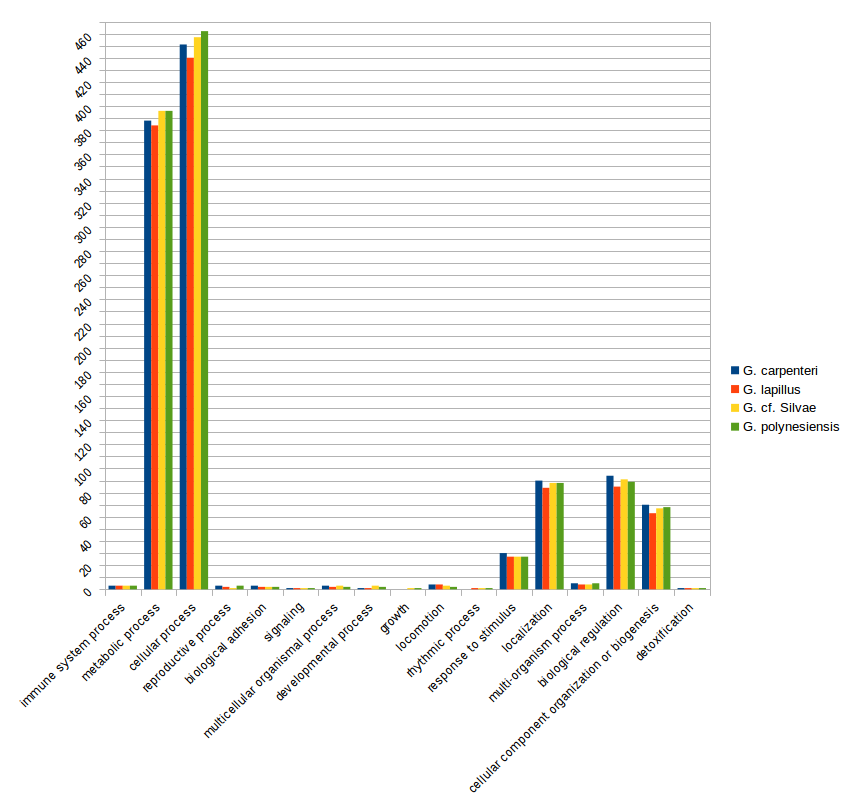
\includegraphics[scale=.78]{3Aug18_cluster-investigation/figures/gosum-species/Species-gosum1-bio.png} 
\caption{Summary of biological processes GO annotations between core, softcore and unique clusters at GOSUM level 1.} 
\label{fig:SpecGo1Bio}
\end{figure} 
\FloatBarrier

\begin{figure} 
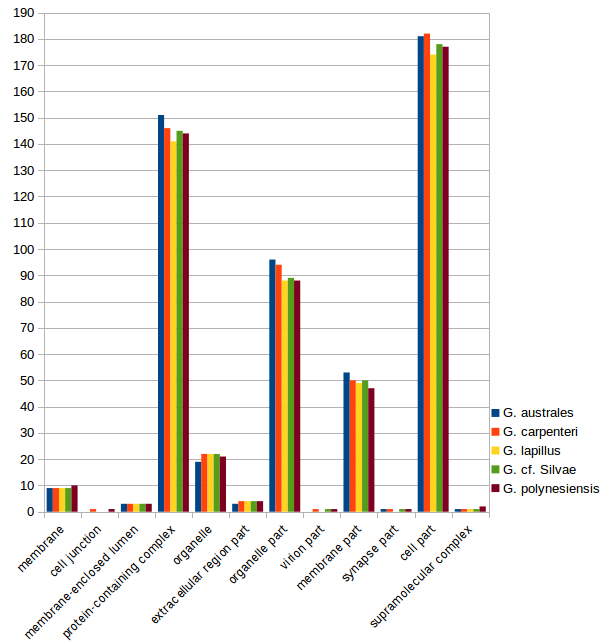
\includegraphics[scale=.8]{3Aug18_cluster-investigation/figures/gosum-species/Species-gosum1-cell.png} 
\caption{Summary of cellular GO annotations between core, softcore and unique clusters at GOSUM level 1.} 
\label{fig:SpecGo1Cell}
\end{figure} 
\FloatBarrier

\begin{figure} 
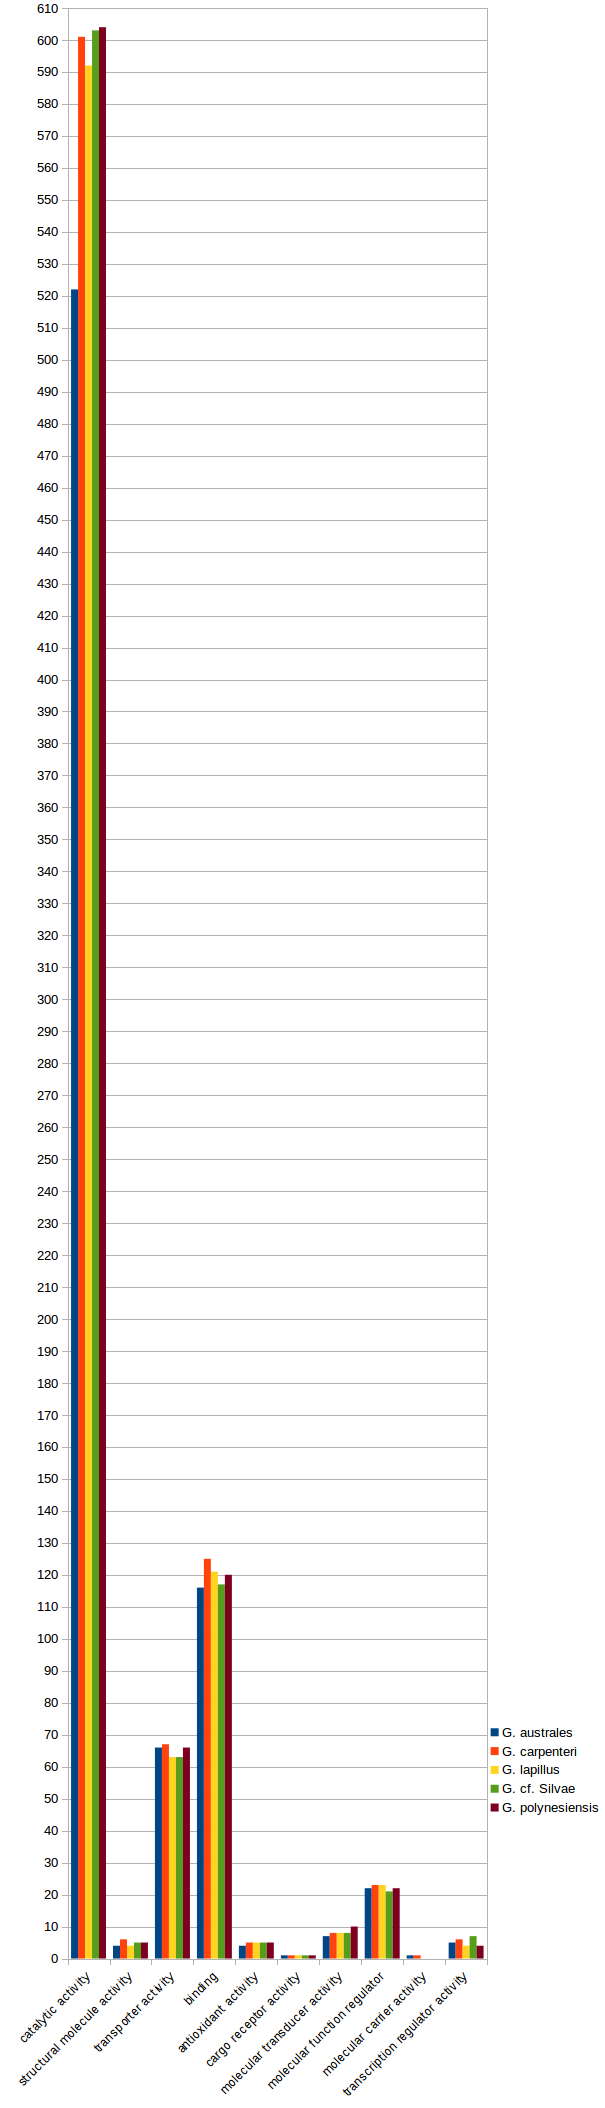
\includegraphics[scale=1]{3Aug18_cluster-investigation/figures/gosum-species/Species-gosum1-molec.png} 
\caption{Summary of molecular GO annotations between core, softcore and unique clusters at GOSUM level 1.} 
\label{fig:SpecGo1Molec}
\end{figure} 
\FloatBarrier

\begin{figure} 
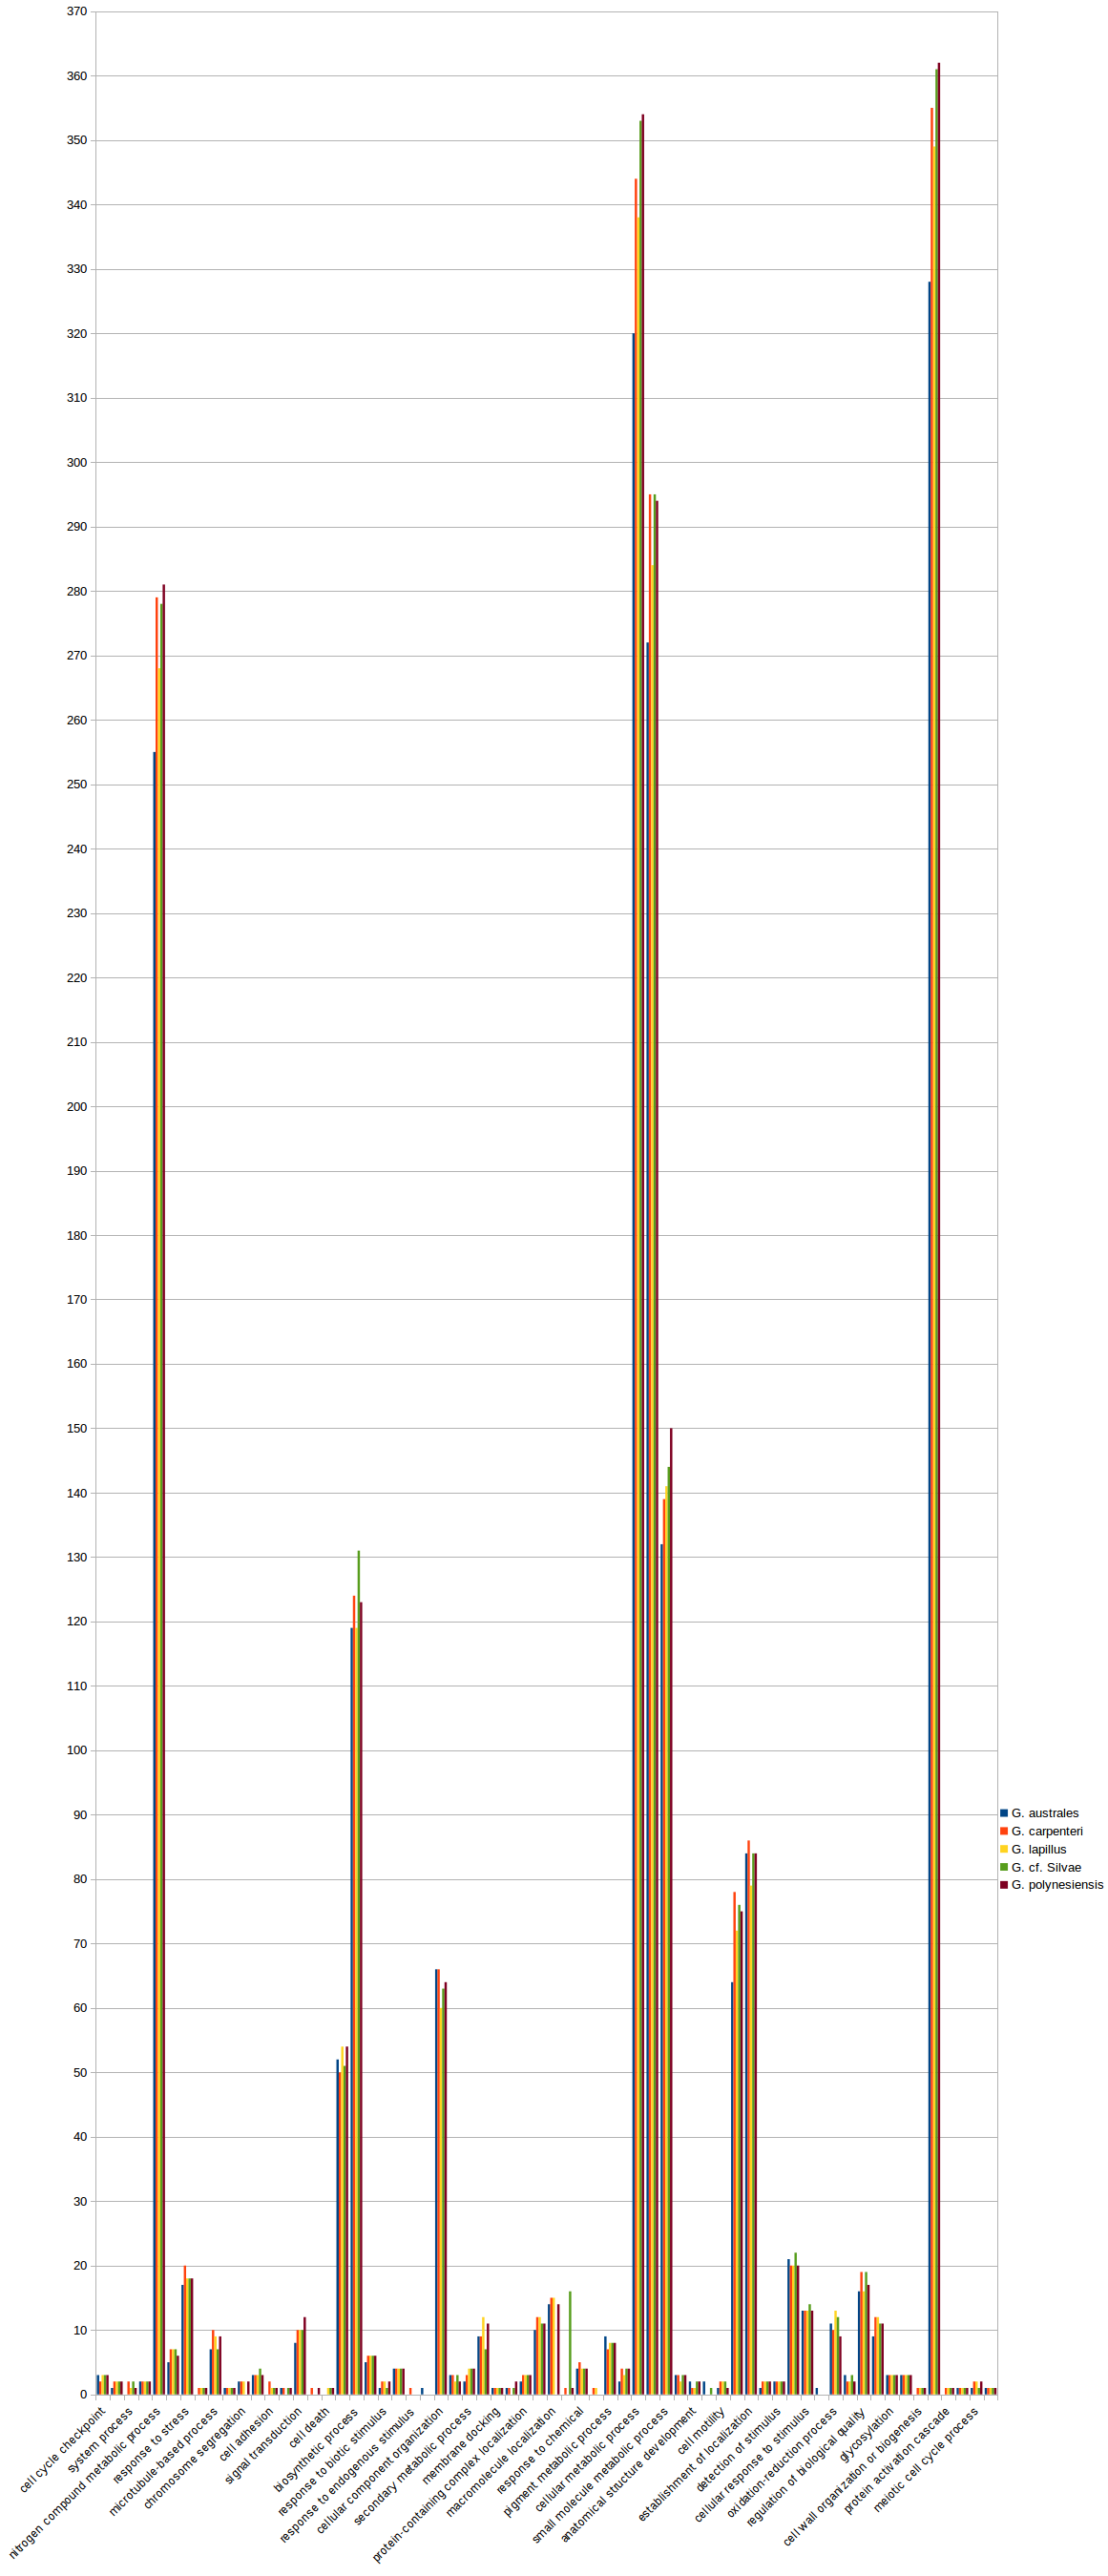
\includegraphics[scale=.9]{3Aug18_cluster-investigation/figures/gosum-species/Species-gosum2-bio.png} 
\caption{Summary of biological processes GO annotations between core, softcore and unique clusters at GOSUM level 2.} 
\label{fig:SpecGo2Bio}
\end{figure} 
\FloatBarrier

\begin{figure} 
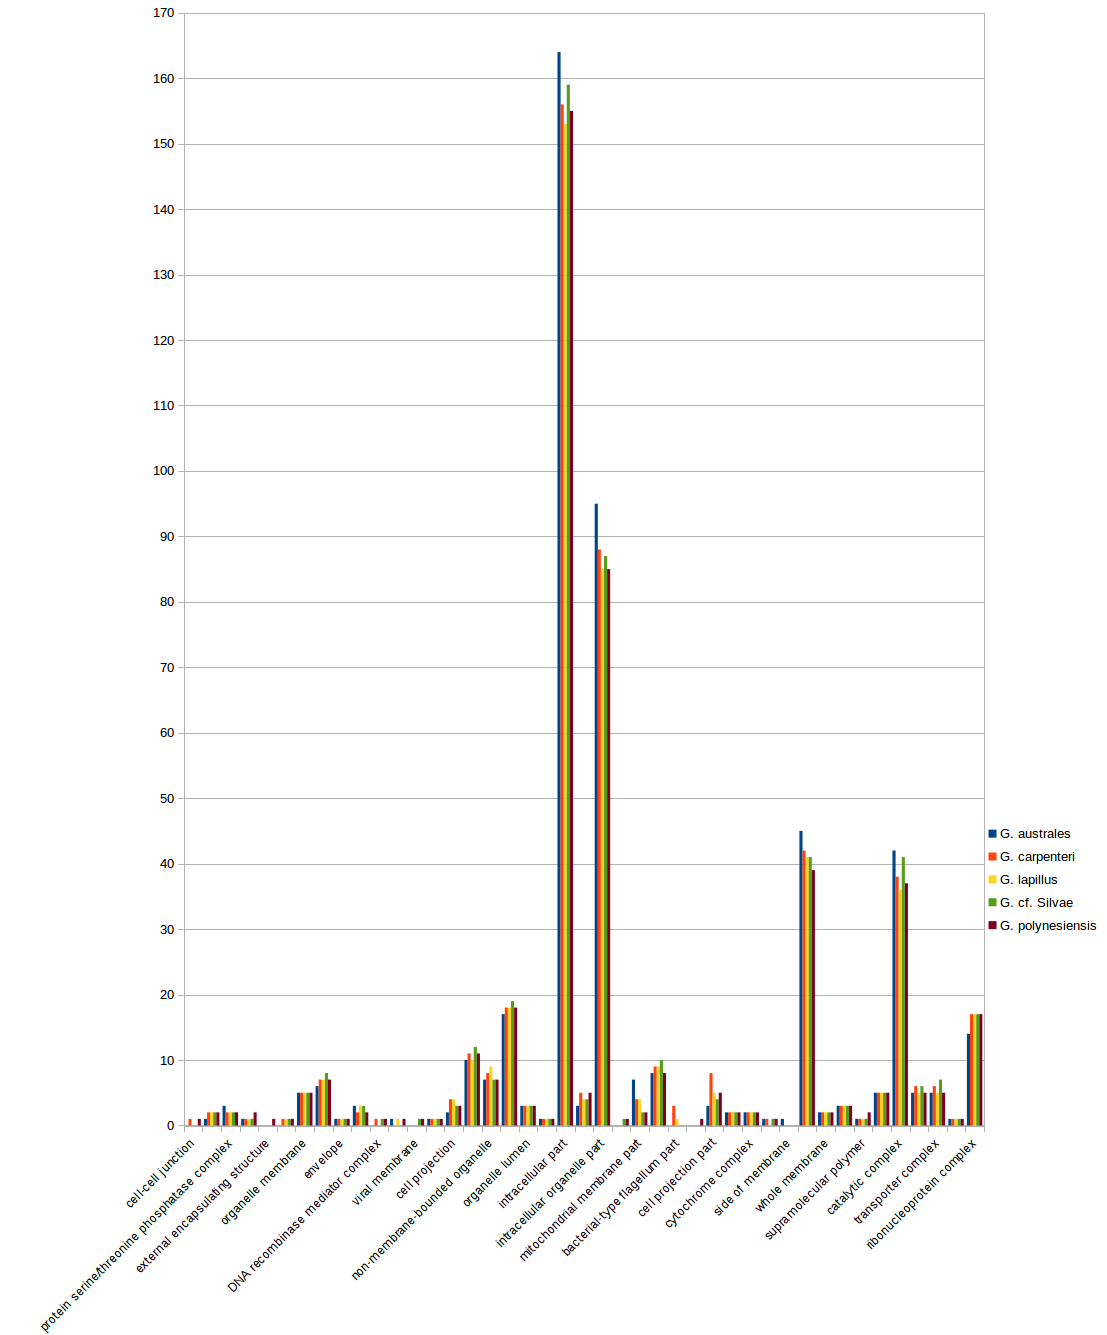
\includegraphics[scale=1]{3Aug18_cluster-investigation/figures/gosum-species/Species-gosum2-cell.png} 
\caption{Summary of cellular GO annotations between core, softcore and unique clusters at GOSUM level 2.} 
\label{fig:SpecGo2Cell}
\end{figure} 
\FloatBarrier

\begin{figure} 
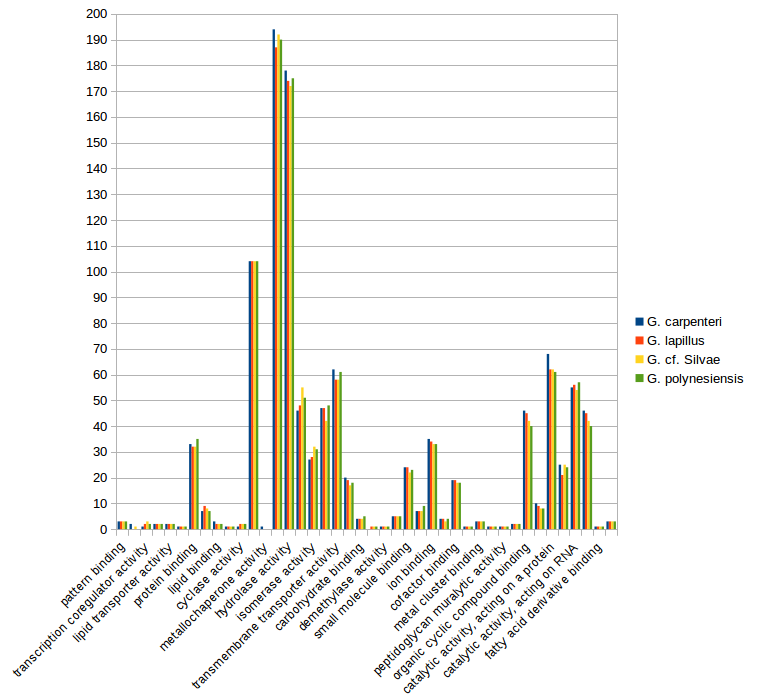
\includegraphics[scale=.85]{3Aug18_cluster-investigation/figures/gosum-species/Species-gosum2-molec.png} 
\caption{Summary of molecular GO annotations between core, softcore and unique clusters at GOSUM level 2.} 
\label{fig:SpecGo2Molec}
\end{figure} 
\FloatBarrier

\subsubsection*{Core transcritome}
- number of clusters\\
- percentage annotated \\
- GOSUM summary \\
- pathways present
\subsubsection*{Softcore - 4 of 5 species}
- number of clusters\\
- percentage annotated \\
- pathways present\\
- which most commonly not present
\subsection*{\emph{Gambierdiscus} inter-species pan-transcriptome}
- which species most commonly solo\\
- number of clusters\\
- percentage annotated \\
- pathways present\\
- any change in contig numbers between species within clusters
\subsubsection*{Unique clusters}
- which species most commonly solo\\
- number of clusters\\
- percentage annotated \\
- pathways present\\


%\subsection*{\emph{Gambierdiscus polynesiensis} intra-species core \& pan transcriptome}
\subsection*{Looking into toxin producers}
\subsubsection*{Clusters with \textit{G. lapillus}, \textit{G. polynesiensis} \& \textit{G. cf. silvae}}
\subsubsection*{\textit{G. polynesiensis solo clusters}}
- number of clusters\\
- percentage annotated \\
- pathways present\\
\subsubsection*{Polyketide synthase genes}
- number of contigs found in each transcriptome\\
- how many clusters do they end up in and what is the proportion of species in there \\
- any multi-domain ones?\\

\begin{table}
\caption{\emph{Gambierdiscus} species transcriptomes used in this study along with their toxicity, toxin profile, accession numbers and source.}
\label{tbl:SeqTable}
\begin{tabular}{ | p{3cm} | p{2cm} | p{2.5cm} | p{2.5cm} | p{2cm} | p{2cm}|}
\hline
\textbf{Species} & \textbf{Source location}&\textbf{LC-MS/MS} & \textbf{Toxicity via bioassay} & \textbf{Accession ID} & \textbf{References} \\
\hline
\textit{Gambierdiscus australes} (CAWD149)&Rarotonga, Cook Islands& CTX -ve; MTX +ve&CTX +ve; MTX N/A&MMETSP0766&\cite{keeling2014marine,rhodes2010toxic,rhodes2014production,munday2017ciguatoxins}\\
\hline
\textit{Gambierdiscus carpenteri} (UTSMER9A)&Merimbula, NSW, Australia&CTX -ve; MTX -ve&CTX -ve; MTX +ve&SRR6821720
&\textbf{chapter 4} \& \cite{larsson2018toxicology}\\
\hline
\textit{Gambierdiscus lapillus} (HG4)&Heron Island, QLD, Australia&CTX -ve; MTX +ve&CTX +ve; MTX +ve&SRR6821722
&\textbf{chapter 4} \& \cite{larsson2018toxicology,kretzschmar2017characterization}\\
\hline
\textit{Gambierdiscus polynesiensis} (CG15)&Rarotonga, Cook Islands&CTX +ve; MTX +ve&CTX N/A; MTX N/A&SRR6821723
&\textbf{chapter 4} \\
\hline
%\textit{Gambierdiscus polynesiensis}&CAWD212&CTX +ve; MTX +ve&CTX N/A; MTX N/A&Kohli pers. comm.&\cite{rhodes2014production}\\
%\hline
%\textit{Gambierdiscus polynesiensis}&CAWD254&CTX -ve; MTX -ve&CTX N/A; MTX N/A&&This study\\
%\hline
\textit{Gambierdiscus} cf. \textit{silvae} (HG5)&Heron Island, QLD, Australia&CTX -ve; MTX +ve&CTX +ve; MTX +ve&SRR6821721
&\textbf{chapter 4} \& \cite{larsson2018toxicology,kretzschmar2017characterization}\\
\hline
\end{tabular}
\end{table}
\FloatBarrier
\newpage
\section*{Discussion}
-overall summary of study

\subsection*{core \textit{Gambierdiscus} transcriptome}
- \cite{lidie2005gene} comprehensive index of genes in K. brevis to compare to 

\subsubsection*{discuss common \& different gene pathways found}

\begin{figure} 
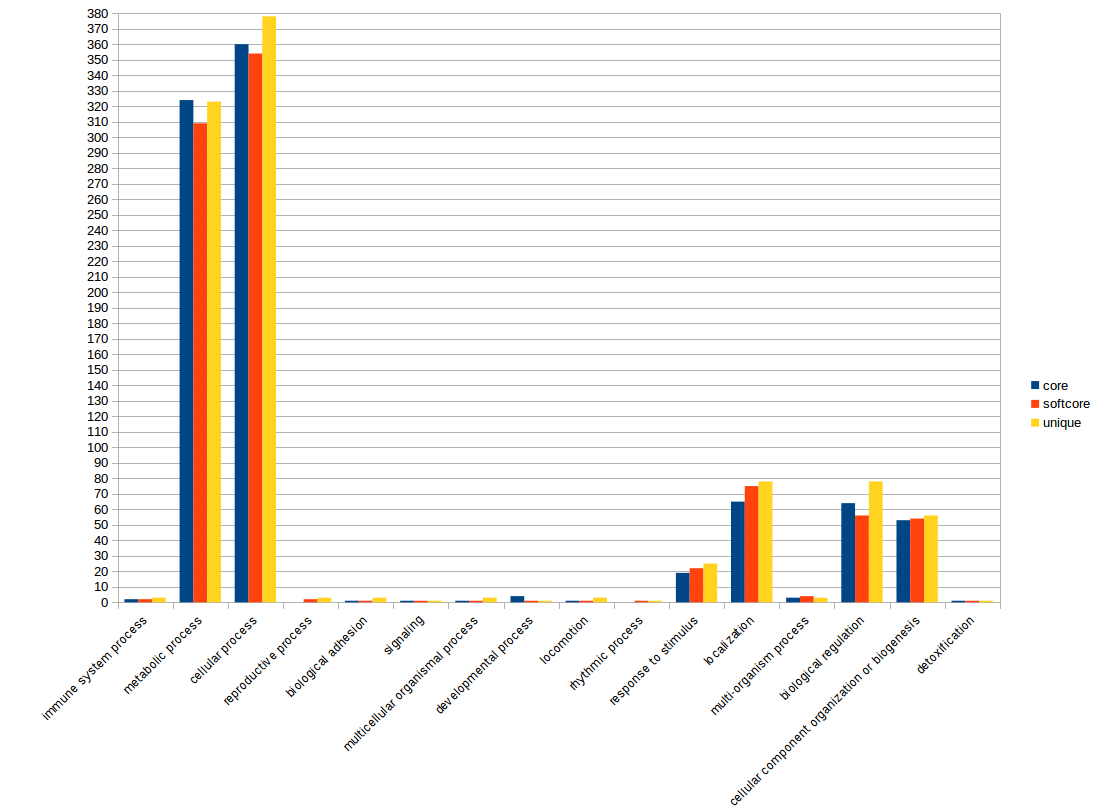
\includegraphics[scale=.6]{3Aug18_cluster-investigation/figures/gosum-pan/Pan-gosum1-bio-graph.png} 
\caption{Summary of biological processes GO annotations between core, softcore and unique clusters at GOSUM level 1.} 
\label{fig:PanGo1Bio}
\end{figure} 
\FloatBarrier

\begin{figure} 
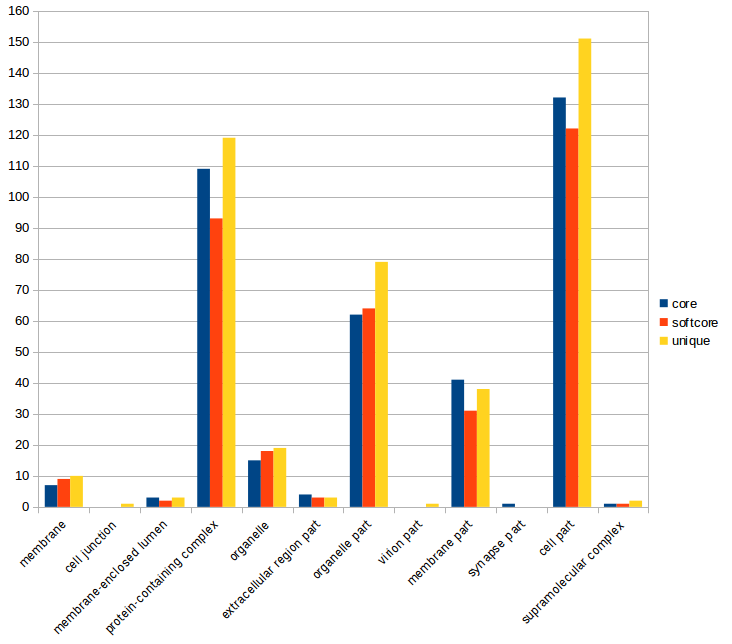
\includegraphics[scale=.8]{3Aug18_cluster-investigation/figures/gosum-pan/Pan-gosum1-cell-graph.png} 
\caption{Summary of cellular GO annotations between core, softcore and unique clusters at GOSUM level 1.} 
\label{fig:PanGo1Cell}
\end{figure} 
\FloatBarrier

\begin{figure} 
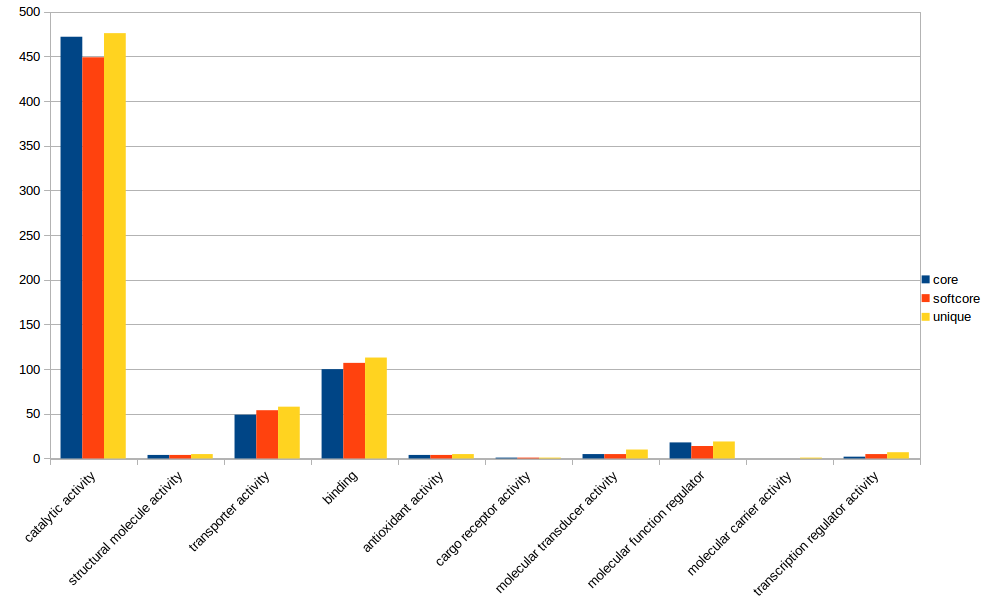
\includegraphics[scale=.65]{3Aug18_cluster-investigation/figures/gosum-pan/Pan-gosum1-molec-graph.png} 
\caption{Summary of molecular GO annotations between core, softcore and unique clusters at GOSUM level 1.} 
\label{fig:PanGo1Molec}
\end{figure} 
\FloatBarrier

\begin{figure} 
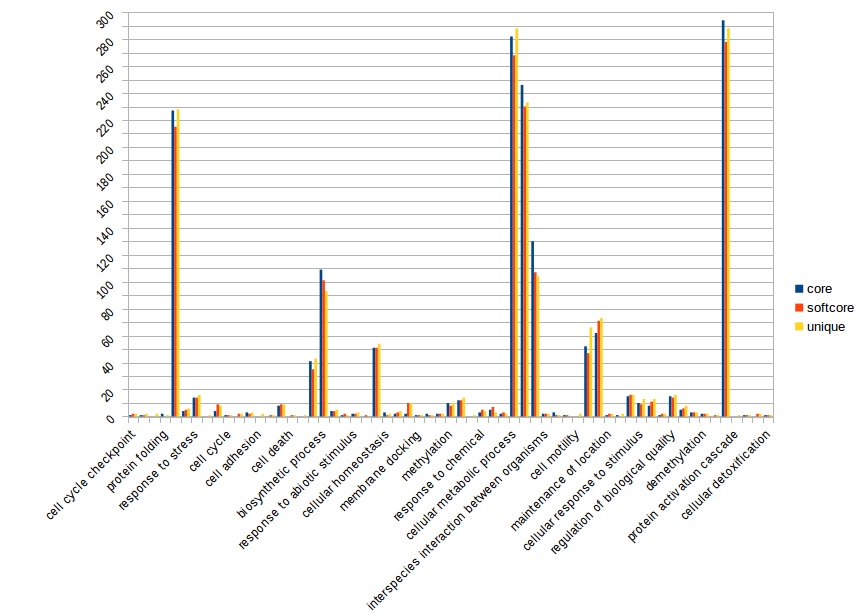
\includegraphics[scale=.75]{3Aug18_cluster-investigation/figures/gosum-pan/Pan-gosum2-bio-graph.png} 
\caption{Summary of biological processes GO annotations between core, softcore and unique clusters at GOSUM level 2.} 
\label{fig:PanGo2Bio}
\end{figure} 
\FloatBarrier

\begin{figure} 
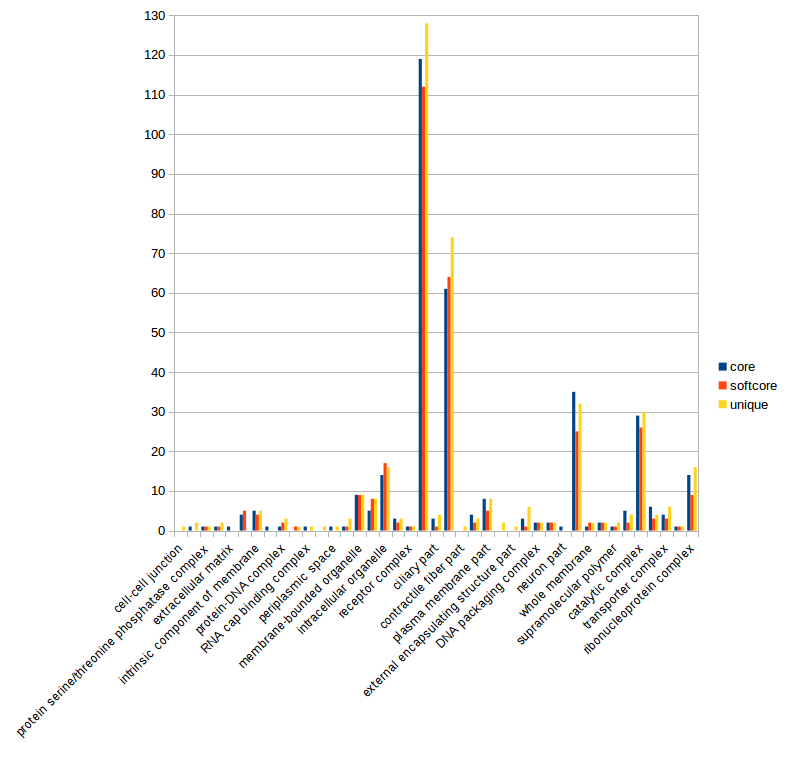
\includegraphics[scale=.8]{3Aug18_cluster-investigation/figures/gosum-pan/Pan-gosum2-cell-graph.png} 
\caption{Summary of cellular GO annotations between core, softcore and unique clusters at GOSUM level 2.} 
\label{fig:PanGo2Cell}
\end{figure} 
\FloatBarrier

\begin{figure} 
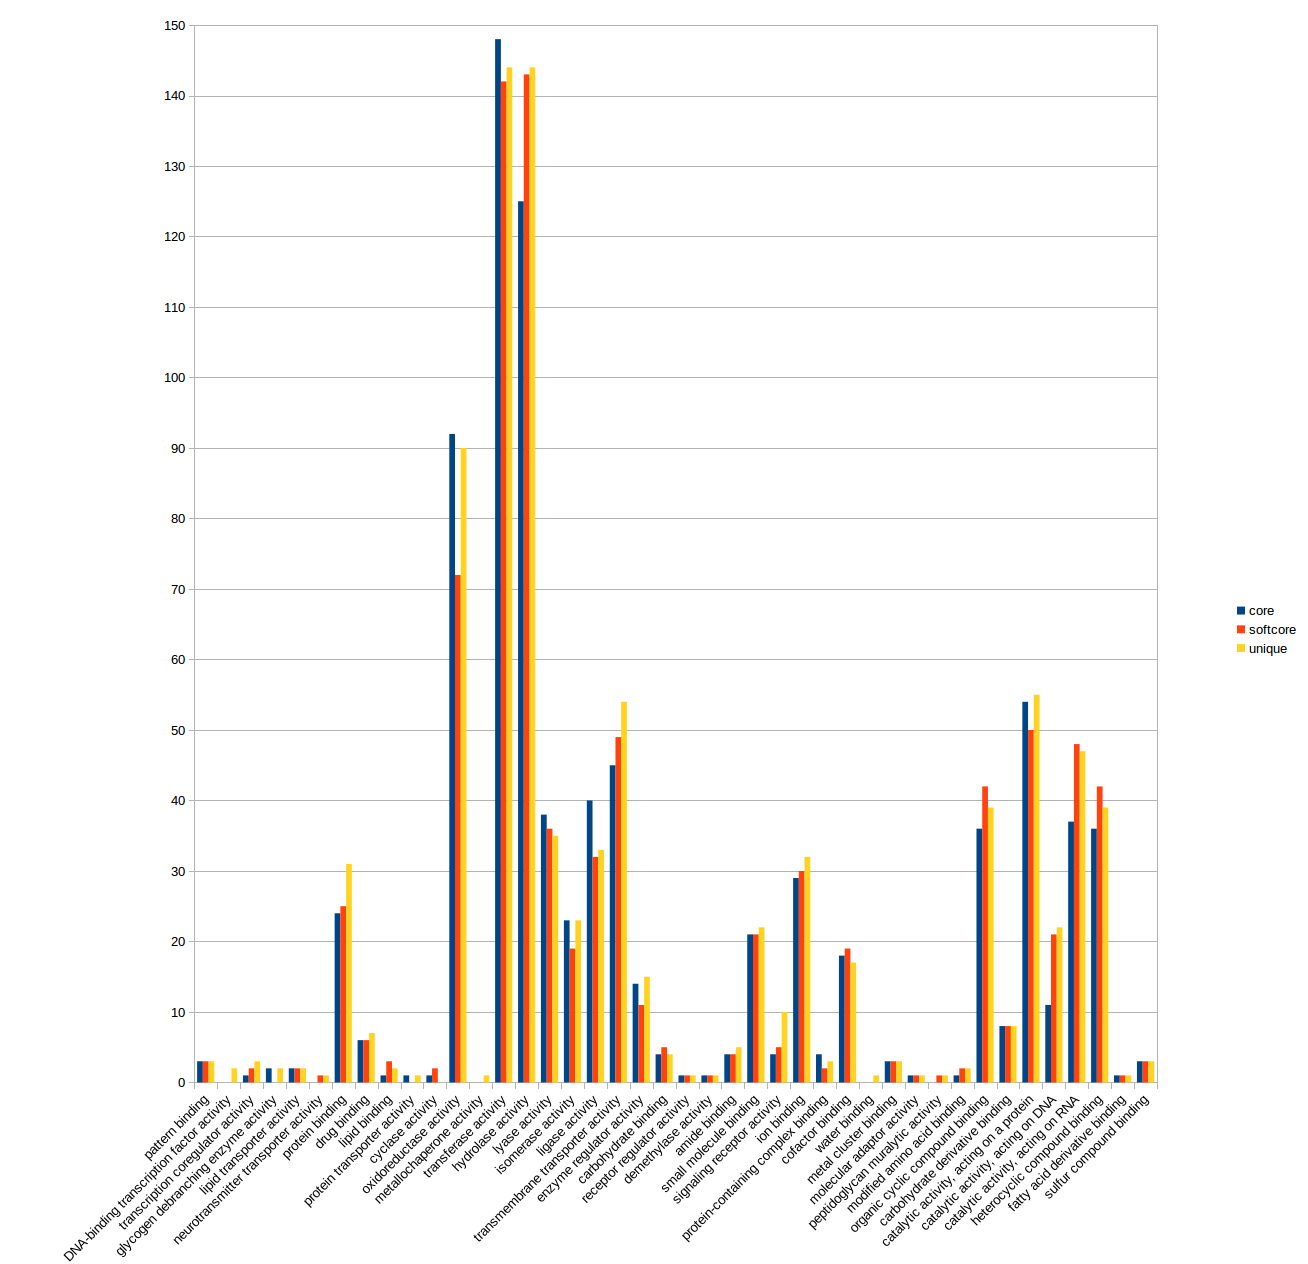
\includegraphics[scale=.6]{3Aug18_cluster-investigation/figures/gosum-pan/Pan-gosum2-molec-graph.png} 
\caption{Summary of molecular GO annotations between core, softcore and unique clusters at GOSUM level 2.} 
\label{fig:PanGo2Molec}
\end{figure} 
\FloatBarrier

\subsubsection*{discuss usefulness for future studies}

\subsubsection*{Expression of genes involved in polyketide production}
- discuss if different gene sets were expressed between toxic and non- toxic strains\\
- discuss if diff genes between all 3 strains\\
- discuss short comings with CAWD254 not having bioassays run, sequencing differences etc

\subsubsection*{discuss potential short commings} 
- from different seq runs and methods and seq depth may vary, especially \textit{G. australes} \\
- intra-speces variation so one isolate per species may not be representative \\
- unknown if processes other than PKS play a role in toxin production
%\subsection*{core \textit{G. polynesiensis} transcriptome}
%- discuss common gene pathways found \\
%-discuss usefulness for future studies\\
%-discuss potential short commings

%\newpage
\section*{Conclusion}


\section*{Supplementary}
- gosum tables with GO annotations


\newpage
\bibliographystyle{acm}
\bibliography{pantran.bib}


\end{document}
